\documentclass[../../../../main.tex]{subfiles}

\begin{document}

\subsection*{第1問}

[解] $P$ が $z=0$ 上 $x^2+y^2=(4a)^2$ の上を運動するとき, $N\left(\frac{1}{2}a, 0, \frac{\sqrt{3}}{2}a\right)$ とする。$N$ での $S$ の接平面は,
\[
\pi : \frac{1}{2}ax + \frac{\sqrt{3}}{2}az = a^2
\]
である。したがって, $\pi$ と $z=0$ の交点は, $x=2a$ となり, 右下図, $P$ が見えるのは, $x \ge 2a$ の領域だから, 見え続ける時間として,
\[
\frac{\pi}{12} \cdot t = \frac{2}{3}\pi \quad \therefore t = 8 \text{ [s]}
\]
である。この時, $C = \cos\theta, S = \sin\theta$ として,
\[
P(4aC, 4aS, 0) \quad \left(-\frac{1}{3}\pi \le \theta \le \frac{1}{3}\pi\right)
\]
とおける。
\[
\overline{NP}^2 = \left(4aC - \frac{1}{2}a\right)^2 + (4aS)^2 + \left(\frac{\sqrt{3}}{2}a\right)^2
\]
\[
\frac{1}{a^2} \overline{NP}^2 = 16C^2 - 4C + \frac{1}{4} + 16S^2 + \frac{3}{4} = -4C + 17
\]
だから, $-\frac{\pi}{3} \le \theta \le \frac{\pi}{3}$ では, $\overline{NP}$ は, $\theta=0$ で $\min 13$, $\theta = \pm \frac{\pi}{3}$ で $\max 15$ をとるから, $\overline{NP} \ge 0$ より,
\[
\begin{cases} \max \overline{NP} = a\sqrt{15} \\ \min \overline{NP} = a\sqrt{13} \end{cases}
\]

\begin{center}
\begin{tikzpicture}[scale=1.0, >=stealth]
  \draw[->] (0,0,0) -- (2.5,0,0) node[right] {$x$};
  \draw[->] (0,0,0) -- (0,2.5,0) node[above] {$z$};
  \draw[->] (0,0,0) -- (-1.5,-1.5,0) node[below left] {$y$};
  \node[below left] at (0,0,0) {$O$};
  
  \draw (0,0) circle (1);
  \coordinate (N) at (0.5, 0.866);
  \fill (N) circle (1.5pt) node[above right] {$N$};
  \draw[dashed] (0,0) -- (N);
  
  \draw[dashed] (1,0,0) arc (0:360:1 and 0.4);
  \draw (0.5,0) -- (0.5,0.866);
  \node[below] at (2,0) {$4a$};
  
  \coordinate (P) at (1.5,-0.8);
  \fill (P) circle (1.5pt) node[below] {$P$};
\end{tikzpicture}
\hspace{1cm}
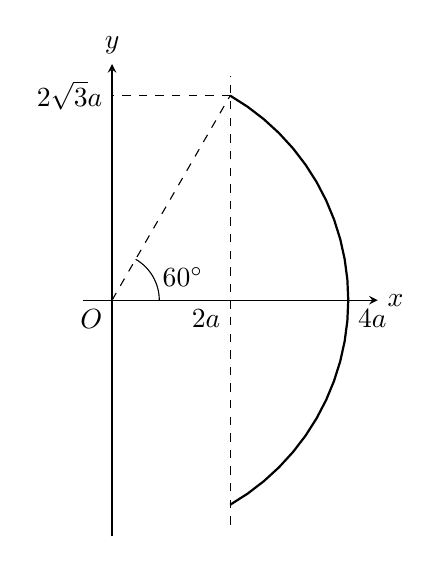
\begin{tikzpicture}[scale=0.75, >=stealth]
  \draw[->] (-0.5,0) -- (4.5,0) node[right] {$x$};
  \draw[->] (0,-4) -- (0,4) node[above] {$y$};
  \node[below left] at (0,0) {$O$};
  
  \draw[dashed] (2,-3.8) -- (2,3.8);
  \node[below left] at (2,0) {$2a$};
  \node[below right] at (4,0) {$4a$};
  
  \draw[thick, domain=-60:60] plot ({4*cos(\x)}, {4*sin(\x)});
  \draw[dashed] (0,0) -- ({4*cos(60)}, {4*sin(60)});
  \draw (0.8,0) arc (0:60:0.8) node[midway, right] {$60^\circ$};
  \node[left] at (0, 3.464) {$2\sqrt{3}a$};
  \draw[dashed] (2, 3.464) -- (0, 3.464);
\end{tikzpicture}
\end{center}

\subsection*{第2問}

[解] $X_i \, (i=1, 2, \dots, n)$ の中に, $0$ が $A$ 個, $1$ が $B$ 個, $2$ が $C$ 個 ($A+B+C=n \dots \phi$) あるとする。
\[
\begin{cases} f_1 = B + 2C \\ f_2 = B + 4C \\ f_k = B + 2^k C \end{cases}
\]
だから, $B, C$ をけして
\[
f_k = (2 - 2^{k-1}) f_1 + (2^{k-1} - 1) f_2
\]

\subsection*{第3問}

[解] $g(x) = f(x) - ax$ とおく。
\[
g(x) = \begin{cases} 1 - ax & (1 \le x \le 2) \\ (1-a)x - 1 & (2 \le x \le 3) \end{cases}
\]
だから, $a$ によって, $V(a)$ は以下のようになる。

$1^\circ$ $a \le 0$ の時\\
$g(x)$ は単調増加で,
\[
V(a) = g(3) - g(1) = 1 - 2a \quad \dots \text{①}
\]

$2^\circ$ $0 \le a \le 1$ の時\\
$g(x)$ のグラフは右図で,
\[
\begin{cases} 0 \le a \le \frac{1}{2} \text{ の時}, & g(3) \ge g(1) \\ \frac{1}{2} \le a \le 1 \text{ の時}, & g(3) \le g(1) \end{cases}
\]
だから
\[
V(a) = \begin{cases} g(3) - g(2) = 1 - a & (0 \le a \le \frac{1}{2}) \\ g(1) - g(2) = a & (\frac{1}{2} \le a \le 1) \end{cases} \quad \dots \text{②}
\]

$3^\circ$ $1 \le a$ の時\\
$g(x)$ は単調減少で,
\[
V(a) = g(1) - g(3) = 2a - 1 \quad \dots \text{③}
\]

したがって, ①〜③から, $V(a)$ は $a = \frac{1}{2}$ で $\min V(a) = \frac{1}{2}$ をとる。
\[
\text{(ii)} \quad a = \frac{1}{2}, \quad \text{(i)} \quad \frac{1}{2}
\]

\begin{center}
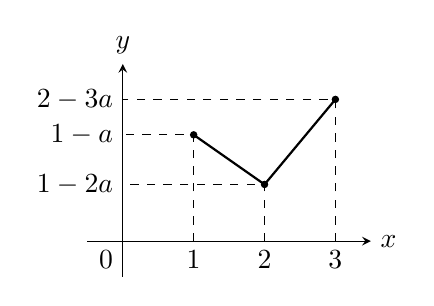
\begin{tikzpicture}[scale=0.9, >=stealth]
  \draw[->] (-0.5,0) -- (3.5,0) node[right] {$x$};
  \draw[->] (0,-0.5) -- (0,2.5) node[above] {$y$};
  \node[below left] at (0,0) {$0$};
  
  \draw[thick] (1,1.5) -- (2,0.8) -- (3,2.0);
  \fill (1,1.5) circle (1.5pt);
  \fill (2,0.8) circle (1.5pt);
  \fill (3,2.0) circle (1.5pt);
  
  \draw[dashed] (1,0) node[below] {$1$} -- (1,1.5) -- (0,1.5) node[left] {$1-a$};
  \draw[dashed] (2,0) node[below] {$2$} -- (2,0.8) -- (0,0.8) node[left] {$1-2a$};
  \draw[dashed] (3,0) node[below] {$3$} -- (3,2.0) -- (0,2.0) node[left] {$2-3a$};
\end{tikzpicture}
\hspace{1cm}
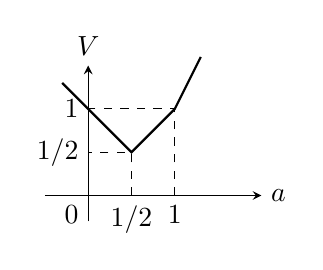
\begin{tikzpicture}[scale=1.1, >=stealth]
  \draw[->] (-0.5,0) -- (2.0,0) node[right] {$a$};
  \draw[->] (0,-0.3) -- (0,1.5) node[above] {$V$};
  \node[below left] at (0,0) {$0$};
  
  \draw[thick] (-0.3, 1.3) -- (0, 1.0) -- (0.5, 0.5) -- (1.0, 1.0) -- (1.3, 1.6);
  
  \draw[dashed] (0.5,0) node[below] {$1/2$} -- (0.5,0.5) -- (0,0.5) node[left] {$1/2$};
  \draw[dashed] (1.0,0) node[below] {$1$} -- (1.0,1.0) -- (0,1.0) node[left] {$1$};
\end{tikzpicture}
\end{center}

\subsection*{第4問}

[解] $P(a,b)$ とおく。対称性から, まず $0 \le a, b$ として考える。 \quad \dots \text{①}

この時 $T(P)$ の周及び内部の点 $(X,Y)$ は
\[
\begin{cases} a - \frac{1}{2} \le X \le a + \frac{1}{2} \\ b - \frac{1}{2} \le Y \le b + \frac{1}{2} \end{cases}
\]
をみたす。これと $S$ が共通部分を持つには,
\[
\begin{cases} a - \frac{1}{2} \le \frac{1}{2} \\ b - \frac{1}{2} \le \frac{1}{2} \end{cases} \iff \begin{cases} a \le 1 \\ b \le 1 \end{cases} \quad \dots \text{②}
\]
が必要。このもとで, 共通部分は,
\[
\begin{cases} a - \frac{1}{2} \le x \le \frac{1}{2} \\ b - \frac{1}{2} \le y \le \frac{1}{2} \end{cases}
\]
で表され, この面積 $T$ は
\[
T = (1-a)(1-b)
\]
である。これが $\frac{1}{2}$ 以上の時,
\[
\frac{1}{2} \le (1-a)(1-b) \quad \dots \text{③}
\]
①, ②, ③に注意して, 求める領域は右図斜線部。\\
(境界含む) ただし, これは $x, y$ 軸に関して対称である。

この面積 $U$ は,
\[
\begin{aligned}
U &= 4 \int_0^{1/2} \left( 1 - \frac{1}{2(1-a)} \right) da \\
&= 4 \left[ a + \frac{1}{2} \log|1-a| \right]_0^{1/2} \\
&= 4 \left[ \frac{1}{2} + \frac{1}{2} \log \frac{1}{2} \right] \\
&= 2(1 - \log 2)
\end{aligned}
\]

\begin{center}
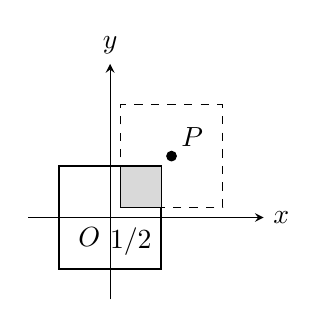
\begin{tikzpicture}[scale=1.3, >=stealth]
  \draw[->] (-0.8,0) -- (1.5,0) node[right] {$x$};
  \draw[->] (0,-0.8) -- (0,1.5) node[above] {$y$};
  \node[below left] at (0,0) {$O$};
  
  \draw[thick] (-0.5,-0.5) rectangle (0.5,0.5);
  \node[below left] at (0.5,0) {$1/2$};
  
  \draw[dashed] (0.1,0.1) rectangle (1.1,1.1);
  \fill (0.6,0.6) circle (1.5pt) node[above right] {$P$};
  
  \fill[gray!30] (0.1,0.1) rectangle (0.5,0.5);
  \draw (0.1,0.1) rectangle (0.5,0.5);
\end{tikzpicture}
\hspace{1cm}
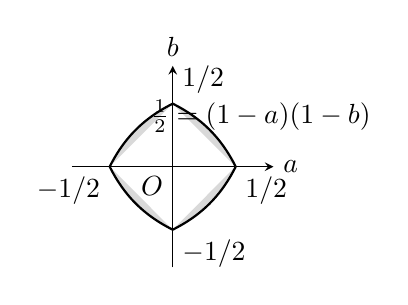
\begin{tikzpicture}[scale=1.6, >=stealth]
  \draw[->] (-0.8,0) -- (0.8,0) node[right] {$a$};
  \draw[->] (0,-0.8) -- (0,0.8) node[above] {$b$};
  \node[below left] at (0,0) {$O$};
  
  \fill[gray!30, domain=0:0.5, samples=50] 
    plot (\x, {1 - 1/(2*(1-\x))}) -- plot (\x, {-1 + 1/(2*(1-\x))}) -- cycle;
  \fill[gray!30, domain=-0.5:0, samples=50] 
    plot (\x, {1 - 1/(2*(1+\x))}) -- plot (\x, {-1 + 1/(2*(1+\x))}) -- cycle;
    
  \draw[thick, domain=0:0.5, samples=50] plot (\x, {1 - 1/(2*(1-\x))});
  \draw[thick, domain=0:0.5, samples=50] plot (\x, {-1 + 1/(2*(1-\x))});
  \draw[thick, domain=-0.5:0, samples=50] plot (\x, {1 - 1/(2*(1+\x))});
  \draw[thick, domain=-0.5:0, samples=50] plot (\x, {-1 + 1/(2*(1+\x))});
  
  \node[below right] at (0.5,0) {$1/2$};
  \node[below left] at (-0.5,0) {$-1/2$};
  \node[above right] at (0,0.5) {$1/2$};
  \node[below right] at (0,-0.5) {$-1/2$};
  \node at (0.7, 0.4) {$\frac{1}{2} = (1-a)(1-b)$};
\end{tikzpicture}
\end{center}

\subsection*{第5問}

[解] $t > 1 \dots \text{①}$ である。(1), (2)を満たす $(x,y)$ は右図斜線部 (境界含む)。したがって
\[
\begin{aligned}
f(t) &= \int_{1/t}^t \left( \frac{1}{1+x^2} - \frac{t}{1+t^2} \frac{1}{x} \right) dx \\
&= \int_{1/t}^t \frac{1}{1+x^2} \, dx - \frac{t}{1+t^2} \int_{1/t}^t \frac{1}{x} \, dx
\end{aligned}
\]
両辺 $t$ で微分して,
\[
\begin{aligned}
f'(t) &= \frac{1}{1+t^2} - \frac{1}{1+(1/t)^2} \left(-\frac{1}{t^2}\right) - \frac{1}{1+t^2} \left( \frac{1}{t} - t \left(-\frac{1}{t^2}\right) \right) - \frac{1-t^2}{(1+t^2)^2} \int_{1/t}^t \frac{1}{x} \, dx \\
&= \frac{1}{1+t^2} + \frac{1}{1+t^2} - \frac{2}{1+t^2} - \frac{1-t^2}{(1+t^2)^2} [\log x]_{1/t}^t \\
&= -\frac{2(1-t^2)}{(1+t^2)^2} \log t
\end{aligned}
\]

\begin{center}
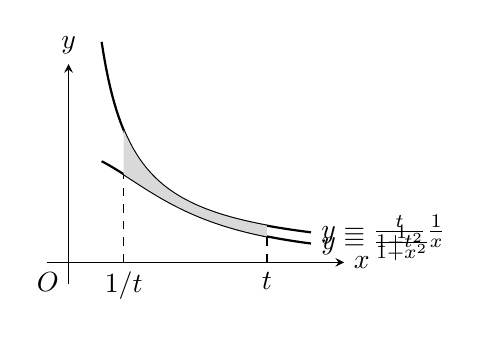
\begin{tikzpicture}[scale=1.4, >=stealth]
  \draw[->] (-0.2,0) -- (2.5,0) node[right] {$x$};
  \draw[->] (0,-0.2) -- (0,1.8) node[above] {$y$};
  \node[below left] at (0,0) {$O$};
  
  \draw[thick, domain=0.3:2.2, samples=100] plot (\x, {1/(1+\x*\x)}) node[right] {$y = \frac{1}{1+x^2}$};
  \draw[thick, domain=0.3:2.2, samples=100] plot (\x, {0.6/\x}) node[right] {$y = \frac{t}{1+t^2}\frac{1}{x}$};
  
  \draw[dashed] (0.5,0) node[below] {$1/t$} -- (0.5, {1/(1+0.25)});
  \draw[dashed] (1.8,0) node[below] {$t$} -- (1.8, {1/(1+1.8*1.8)});
  
  \fill[gray!30, domain=0.5:1.8, samples=50]
    plot (\x, {1/(1+\x*\x)}) -- plot (2.3-\x, {0.6/(2.3-\x)}) -- cycle;
\end{tikzpicture}
\end{center}

\subsection*{第6問}

[解] 題意の放物線を $y = f(x) = ax^2 + bx$ ($a \neq 0$) とおく。($\because f(0)=0$)

$f'(0) = 1$ だから, $b = 1$ なので
\[
f(x) = ax^2 + x
\]
\[
\therefore f'(x) = 2ax + 1
\]
だから, グラフ上の点 $(u, v)$ での接線の傾きは, $\left( a = \frac{v-u}{u^2} \text{ より} \right)$
\[
f'(u) = 2u \frac{v-u}{u^2} + 1 = \frac{2v-u}{u} \quad (\because u \neq 0)
\]

\end{document}
